\documentclass[aspectratio=169]{beamer}

\usetheme{Boadilla}
\usefonttheme{professionalfonts}
\setbeamertemplate{navigation symbols}{}
\setbeamertemplate{itemize items}[circle]
\setbeamertemplate{enumerate items}[default]
\setbeamertemplate{headline}{}

\usepackage[utf8]{inputenc}
\usepackage[T1]{fontenc}
\usepackage{lmodern}
\usepackage{amsmath}
\usepackage{booktabs}
\usepackage{tabularx}
\usepackage{array}
\usepackage{hyperref}
\usepackage[strings]{underscore}
\usepackage{listings}
\usepackage{tikz}
\usetikzlibrary{arrows.meta,positioning,fit,calc,shapes.geometric}
\usepackage{xcolor}

\definecolor{courseblue}{HTML}{12355B}
\definecolor{coursegold}{HTML}{C98A2E}
\definecolor{courseice}{HTML}{EEF3F8}
\definecolor{coursegreen}{HTML}{2F6B4F}
\definecolor{coursegray}{HTML}{4B5563}
\definecolor{codebg}{HTML}{F7F9FC}
\definecolor{codecomment}{HTML}{5E6C84}
\definecolor{codestring}{HTML}{0B6E4F}

\setbeamercolor{palette primary}{bg=courseblue,fg=white}
\setbeamercolor{palette secondary}{bg=coursegold,fg=white}
\setbeamercolor{palette tertiary}{bg=courseblue,fg=white}
\setbeamercolor{palette quaternary}{bg=coursegold,fg=white}
\setbeamercolor{structure}{fg=courseblue}
\setbeamercolor{frametitle}{bg=courseice,fg=courseblue}
\setbeamercolor{title}{fg=courseblue}
\setbeamercolor{block title}{bg=courseblue,fg=white}
\setbeamercolor{block body}{bg=courseice,fg=black}
\setbeamercolor{normal text}{fg=black,bg=white}
\setbeamercolor{alerted text}{fg=coursegold}

\setbeamerfont{footline}{size=\scriptsize}

\setbeamertemplate{footline}{
  \leavevmode
  \hbox{
    \begin{beamercolorbox}[wd=.33\paperwidth,ht=2.8ex,dp=1.2ex,leftskip=0.8em]{palette primary}%
      University of Trieste
    \end{beamercolorbox}%
    \begin{beamercolorbox}[wd=.49\paperwidth,ht=2.8ex,dp=1.2ex,center]{palette tertiary}%
      \coursename{} \textbar{} \coursecode
    \end{beamercolorbox}%
    \begin{beamercolorbox}[wd=.18\paperwidth,ht=2.8ex,dp=1.2ex,rightskip=0.8em plus1fil]{palette secondary}%
      \insertframenumber{} / \inserttotalframenumber
    \end{beamercolorbox}%
  }
}

\hypersetup{
  colorlinks=true,
  linkcolor=courseblue,
  urlcolor=coursegreen
}

\lstdefinestyle{coursepython}{
  language=Python,
  basicstyle=\ttfamily\footnotesize,
  keywordstyle=\color{courseblue}\bfseries,
  commentstyle=\color{codecomment}\itshape,
  stringstyle=\color{codestring},
  showstringspaces=false,
  columns=fullflexible,
  keepspaces=true,
  frame=single,
  framerule=0.6pt,
  rulecolor=\color{courseblue},
  backgroundcolor=\color{codebg},
  xleftmargin=0.4em,
  xrightmargin=0.4em,
  aboveskip=0.4em,
  belowskip=0.2em
}

\newcommand{\coursename}{Data-driven Systems Engineering}
\newcommand{\coursecode}{440MI / 305SM}
\newcommand{\coursefooter}{}

\newcommand{\learninggoals}[1]{
  \begin{block}{Learning goals}
  #1
  \end{block}
}

\newcommand{\repoactivity}[1]{
  \begin{block}{Repo activity}
  #1
  \end{block}
}

\newcommand{\readinglist}[1]{
  \begin{block}{Papers and materials}
  {\footnotesize #1}
  \end{block}
}

\newcommand{\coursecontextframe}[5]{
  \begin{frame}{Course Map and Running Cases}
  \centering
  \begin{tikzpicture}[node distance=0.28cm]
  \node[flowbox, minimum width=1.45cm, minimum height=0.8cm] (problem) {\scriptsize Problem};
  \node[flowbox, minimum width=1.45cm, minimum height=0.8cm, right=of problem] (data) {\scriptsize Data};
  \node[flowbox, minimum width=1.45cm, minimum height=0.8cm, right=of data] (features) {\scriptsize Features};
  \node[flowbox, minimum width=1.45cm, minimum height=0.8cm, right=of features] (model) {\scriptsize Model};
  \node[flowbox, minimum width=1.45cm, minimum height=0.8cm, right=of model] (interface) {\scriptsize Interface};
  \node[flowbox, minimum width=1.45cm, minimum height=0.8cm, right=of interface] (delivery) {\scriptsize Delivery};
  \node[flowbox, minimum width=1.45cm, minimum height=0.8cm, right=of delivery] (monitor) {\scriptsize Monitor};
  \node[accentbox, minimum width=1.6cm, minimum height=0.8cm, right=of monitor] (evolution) {\scriptsize Evolution};
  \foreach \a/\b in {problem/data,data/features,features/model,model/interface,interface/delivery,delivery/monitor,monitor/evolution} {
    \draw[arrow] (\a) -- (\b);
  }
  \end{tikzpicture}

  \vspace{0.5em}
  \begin{block}{Today in the course}
  \textbf{Focus:} #1

  \textbf{Bridge:} #2
  \end{block}

  \begin{columns}[T]
  \column{0.48\textwidth}
  \begin{block}{Fraud case}
  {\footnotesize #3}
  \end{block}
  \column{0.48\textwidth}
  \begin{block}{Pasteurization case}
  {\footnotesize #4}
  \end{block}
  \end{columns}

  \vspace{0.3em}
  {\footnotesize \textbf{Course thread:} #5}
  \coursefooter
  \end{frame}
}

\newcommand{\classclosingframe}[4]{
  \begin{frame}{From This Class to the Next}
  \begin{block}{What stays with us}
  #1
  \end{block}

  \begin{columns}[T]
  \column{0.48\textwidth}
  \begin{block}{Project use}
  {\footnotesize #2}
  \end{block}
  \column{0.48\textwidth}
  \begin{block}{Next connection}
  {\footnotesize #3}
  \end{block}
  \end{columns}

  \vspace{0.3em}
  {\footnotesize \textbf{Course thread:} #4}
  \coursefooter
  \end{frame}
}

\tikzset{
  flowbox/.style={
    rounded corners=3pt,
    draw=courseblue,
    fill=courseice,
    very thick,
    minimum width=2.2cm,
    minimum height=0.9cm,
    align=center,
    font=\small
  },
  accentbox/.style={
    rounded corners=3pt,
    draw=coursegold,
    fill=coursegold!15,
    very thick,
    minimum width=2.2cm,
    minimum height=0.9cm,
    align=center,
    font=\small
  },
  arrow/.style={
    -{Latex[length=2.5mm,width=2mm]},
    thick,
    draw=courseblue
  }
}

% Visual layer on top of common.tex: tiles, icons, a progress-strip section divider, and a footer
% strip that defines the concepts appearing for the first time on each slide.
% Same look as the Class 20 deck. Load with:  \documentclass[aspectratio=169]{beamer}

\usetheme{Boadilla}
\usefonttheme{professionalfonts}
\setbeamertemplate{navigation symbols}{}
\setbeamertemplate{itemize items}[circle]
\setbeamertemplate{enumerate items}[default]
\setbeamertemplate{headline}{}

\usepackage[utf8]{inputenc}
\usepackage[T1]{fontenc}
\usepackage{lmodern}
\usepackage{amsmath}
\usepackage{booktabs}
\usepackage{tabularx}
\usepackage{array}
\usepackage{hyperref}
\usepackage[strings]{underscore}
\usepackage{listings}
\usepackage{tikz}
\usetikzlibrary{arrows.meta,positioning,fit,calc,shapes.geometric}
\usepackage{xcolor}

\definecolor{courseblue}{HTML}{12355B}
\definecolor{coursegold}{HTML}{C98A2E}
\definecolor{courseice}{HTML}{EEF3F8}
\definecolor{coursegreen}{HTML}{2F6B4F}
\definecolor{coursegray}{HTML}{4B5563}
\definecolor{codebg}{HTML}{F7F9FC}
\definecolor{codecomment}{HTML}{5E6C84}
\definecolor{codestring}{HTML}{0B6E4F}

\setbeamercolor{palette primary}{bg=courseblue,fg=white}
\setbeamercolor{palette secondary}{bg=coursegold,fg=white}
\setbeamercolor{palette tertiary}{bg=courseblue,fg=white}
\setbeamercolor{palette quaternary}{bg=coursegold,fg=white}
\setbeamercolor{structure}{fg=courseblue}
\setbeamercolor{frametitle}{bg=courseice,fg=courseblue}
\setbeamercolor{title}{fg=courseblue}
\setbeamercolor{block title}{bg=courseblue,fg=white}
\setbeamercolor{block body}{bg=courseice,fg=black}
\setbeamercolor{normal text}{fg=black,bg=white}
\setbeamercolor{alerted text}{fg=coursegold}

\setbeamerfont{footline}{size=\scriptsize}

\setbeamertemplate{footline}{
  \leavevmode
  \hbox{
    \begin{beamercolorbox}[wd=.33\paperwidth,ht=2.8ex,dp=1.2ex,leftskip=0.8em]{palette primary}%
      University of Trieste
    \end{beamercolorbox}%
    \begin{beamercolorbox}[wd=.49\paperwidth,ht=2.8ex,dp=1.2ex,center]{palette tertiary}%
      \coursename{} \textbar{} \coursecode
    \end{beamercolorbox}%
    \begin{beamercolorbox}[wd=.18\paperwidth,ht=2.8ex,dp=1.2ex,rightskip=0.8em plus1fil]{palette secondary}%
      \insertframenumber{} / \inserttotalframenumber
    \end{beamercolorbox}%
  }
}

\hypersetup{
  colorlinks=true,
  linkcolor=courseblue,
  urlcolor=coursegreen
}

\lstdefinestyle{coursepython}{
  language=Python,
  basicstyle=\ttfamily\footnotesize,
  keywordstyle=\color{courseblue}\bfseries,
  commentstyle=\color{codecomment}\itshape,
  stringstyle=\color{codestring},
  showstringspaces=false,
  columns=fullflexible,
  keepspaces=true,
  frame=single,
  framerule=0.6pt,
  rulecolor=\color{courseblue},
  backgroundcolor=\color{codebg},
  xleftmargin=0.4em,
  xrightmargin=0.4em,
  aboveskip=0.4em,
  belowskip=0.2em
}

\newcommand{\coursename}{Data-driven Systems Engineering}
\newcommand{\coursecode}{440MI / 305SM}
\newcommand{\coursefooter}{}

\newcommand{\learninggoals}[1]{
  \begin{block}{Learning goals}
  #1
  \end{block}
}

\newcommand{\repoactivity}[1]{
  \begin{block}{Repo activity}
  #1
  \end{block}
}

\newcommand{\readinglist}[1]{
  \begin{block}{Papers and materials}
  {\footnotesize #1}
  \end{block}
}

\newcommand{\coursecontextframe}[5]{
  \begin{frame}{Course Map and Running Cases}
  \centering
  \begin{tikzpicture}[node distance=0.28cm]
  \node[flowbox, minimum width=1.45cm, minimum height=0.8cm] (problem) {\scriptsize Problem};
  \node[flowbox, minimum width=1.45cm, minimum height=0.8cm, right=of problem] (data) {\scriptsize Data};
  \node[flowbox, minimum width=1.45cm, minimum height=0.8cm, right=of data] (features) {\scriptsize Features};
  \node[flowbox, minimum width=1.45cm, minimum height=0.8cm, right=of features] (model) {\scriptsize Model};
  \node[flowbox, minimum width=1.45cm, minimum height=0.8cm, right=of model] (interface) {\scriptsize Interface};
  \node[flowbox, minimum width=1.45cm, minimum height=0.8cm, right=of interface] (delivery) {\scriptsize Delivery};
  \node[flowbox, minimum width=1.45cm, minimum height=0.8cm, right=of delivery] (monitor) {\scriptsize Monitor};
  \node[accentbox, minimum width=1.6cm, minimum height=0.8cm, right=of monitor] (evolution) {\scriptsize Evolution};
  \foreach \a/\b in {problem/data,data/features,features/model,model/interface,interface/delivery,delivery/monitor,monitor/evolution} {
    \draw[arrow] (\a) -- (\b);
  }
  \end{tikzpicture}

  \vspace{0.5em}
  \begin{block}{Today in the course}
  \textbf{Focus:} #1

  \textbf{Bridge:} #2
  \end{block}

  \begin{columns}[T]
  \column{0.48\textwidth}
  \begin{block}{Fraud case}
  {\footnotesize #3}
  \end{block}
  \column{0.48\textwidth}
  \begin{block}{Pasteurization case}
  {\footnotesize #4}
  \end{block}
  \end{columns}

  \vspace{0.3em}
  {\footnotesize \textbf{Course thread:} #5}
  \coursefooter
  \end{frame}
}

\newcommand{\classclosingframe}[4]{
  \begin{frame}{From This Class to the Next}
  \begin{block}{What stays with us}
  #1
  \end{block}

  \begin{columns}[T]
  \column{0.48\textwidth}
  \begin{block}{Project use}
  {\footnotesize #2}
  \end{block}
  \column{0.48\textwidth}
  \begin{block}{Next connection}
  {\footnotesize #3}
  \end{block}
  \end{columns}

  \vspace{0.3em}
  {\footnotesize \textbf{Course thread:} #4}
  \coursefooter
  \end{frame}
}

\tikzset{
  flowbox/.style={
    rounded corners=3pt,
    draw=courseblue,
    fill=courseice,
    very thick,
    minimum width=2.2cm,
    minimum height=0.9cm,
    align=center,
    font=\small
  },
  accentbox/.style={
    rounded corners=3pt,
    draw=coursegold,
    fill=coursegold!15,
    very thick,
    minimum width=2.2cm,
    minimum height=0.9cm,
    align=center,
    font=\small
  },
  arrow/.style={
    -{Latex[length=2.5mm,width=2mm]},
    thick,
    draw=courseblue
  }
}
  % Visual layer on top of common.tex: tiles, icons, a progress-strip section divider, and a footer
% strip that defines the concepts appearing for the first time on each slide.
% Same look as the Class 20 deck. Load with:  \documentclass[aspectratio=169]{beamer}

\usetheme{Boadilla}
\usefonttheme{professionalfonts}
\setbeamertemplate{navigation symbols}{}
\setbeamertemplate{itemize items}[circle]
\setbeamertemplate{enumerate items}[default]
\setbeamertemplate{headline}{}

\usepackage[utf8]{inputenc}
\usepackage[T1]{fontenc}
\usepackage{lmodern}
\usepackage{amsmath}
\usepackage{booktabs}
\usepackage{tabularx}
\usepackage{array}
\usepackage{hyperref}
\usepackage[strings]{underscore}
\usepackage{listings}
\usepackage{tikz}
\usetikzlibrary{arrows.meta,positioning,fit,calc,shapes.geometric}
\usepackage{xcolor}

\definecolor{courseblue}{HTML}{12355B}
\definecolor{coursegold}{HTML}{C98A2E}
\definecolor{courseice}{HTML}{EEF3F8}
\definecolor{coursegreen}{HTML}{2F6B4F}
\definecolor{coursegray}{HTML}{4B5563}
\definecolor{codebg}{HTML}{F7F9FC}
\definecolor{codecomment}{HTML}{5E6C84}
\definecolor{codestring}{HTML}{0B6E4F}

\setbeamercolor{palette primary}{bg=courseblue,fg=white}
\setbeamercolor{palette secondary}{bg=coursegold,fg=white}
\setbeamercolor{palette tertiary}{bg=courseblue,fg=white}
\setbeamercolor{palette quaternary}{bg=coursegold,fg=white}
\setbeamercolor{structure}{fg=courseblue}
\setbeamercolor{frametitle}{bg=courseice,fg=courseblue}
\setbeamercolor{title}{fg=courseblue}
\setbeamercolor{block title}{bg=courseblue,fg=white}
\setbeamercolor{block body}{bg=courseice,fg=black}
\setbeamercolor{normal text}{fg=black,bg=white}
\setbeamercolor{alerted text}{fg=coursegold}

\setbeamerfont{footline}{size=\scriptsize}

\setbeamertemplate{footline}{
  \leavevmode
  \hbox{
    \begin{beamercolorbox}[wd=.33\paperwidth,ht=2.8ex,dp=1.2ex,leftskip=0.8em]{palette primary}%
      University of Trieste
    \end{beamercolorbox}%
    \begin{beamercolorbox}[wd=.49\paperwidth,ht=2.8ex,dp=1.2ex,center]{palette tertiary}%
      \coursename{} \textbar{} \coursecode
    \end{beamercolorbox}%
    \begin{beamercolorbox}[wd=.18\paperwidth,ht=2.8ex,dp=1.2ex,rightskip=0.8em plus1fil]{palette secondary}%
      \insertframenumber{} / \inserttotalframenumber
    \end{beamercolorbox}%
  }
}

\hypersetup{
  colorlinks=true,
  linkcolor=courseblue,
  urlcolor=coursegreen
}

\lstdefinestyle{coursepython}{
  language=Python,
  basicstyle=\ttfamily\footnotesize,
  keywordstyle=\color{courseblue}\bfseries,
  commentstyle=\color{codecomment}\itshape,
  stringstyle=\color{codestring},
  showstringspaces=false,
  columns=fullflexible,
  keepspaces=true,
  frame=single,
  framerule=0.6pt,
  rulecolor=\color{courseblue},
  backgroundcolor=\color{codebg},
  xleftmargin=0.4em,
  xrightmargin=0.4em,
  aboveskip=0.4em,
  belowskip=0.2em
}

\newcommand{\coursename}{Data-driven Systems Engineering}
\newcommand{\coursecode}{440MI / 305SM}
\newcommand{\coursefooter}{}

\newcommand{\learninggoals}[1]{
  \begin{block}{Learning goals}
  #1
  \end{block}
}

\newcommand{\repoactivity}[1]{
  \begin{block}{Repo activity}
  #1
  \end{block}
}

\newcommand{\readinglist}[1]{
  \begin{block}{Papers and materials}
  {\footnotesize #1}
  \end{block}
}

\newcommand{\coursecontextframe}[5]{
  \begin{frame}{Course Map and Running Cases}
  \centering
  \begin{tikzpicture}[node distance=0.28cm]
  \node[flowbox, minimum width=1.45cm, minimum height=0.8cm] (problem) {\scriptsize Problem};
  \node[flowbox, minimum width=1.45cm, minimum height=0.8cm, right=of problem] (data) {\scriptsize Data};
  \node[flowbox, minimum width=1.45cm, minimum height=0.8cm, right=of data] (features) {\scriptsize Features};
  \node[flowbox, minimum width=1.45cm, minimum height=0.8cm, right=of features] (model) {\scriptsize Model};
  \node[flowbox, minimum width=1.45cm, minimum height=0.8cm, right=of model] (interface) {\scriptsize Interface};
  \node[flowbox, minimum width=1.45cm, minimum height=0.8cm, right=of interface] (delivery) {\scriptsize Delivery};
  \node[flowbox, minimum width=1.45cm, minimum height=0.8cm, right=of delivery] (monitor) {\scriptsize Monitor};
  \node[accentbox, minimum width=1.6cm, minimum height=0.8cm, right=of monitor] (evolution) {\scriptsize Evolution};
  \foreach \a/\b in {problem/data,data/features,features/model,model/interface,interface/delivery,delivery/monitor,monitor/evolution} {
    \draw[arrow] (\a) -- (\b);
  }
  \end{tikzpicture}

  \vspace{0.5em}
  \begin{block}{Today in the course}
  \textbf{Focus:} #1

  \textbf{Bridge:} #2
  \end{block}

  \begin{columns}[T]
  \column{0.48\textwidth}
  \begin{block}{Fraud case}
  {\footnotesize #3}
  \end{block}
  \column{0.48\textwidth}
  \begin{block}{Pasteurization case}
  {\footnotesize #4}
  \end{block}
  \end{columns}

  \vspace{0.3em}
  {\footnotesize \textbf{Course thread:} #5}
  \coursefooter
  \end{frame}
}

\newcommand{\classclosingframe}[4]{
  \begin{frame}{From This Class to the Next}
  \begin{block}{What stays with us}
  #1
  \end{block}

  \begin{columns}[T]
  \column{0.48\textwidth}
  \begin{block}{Project use}
  {\footnotesize #2}
  \end{block}
  \column{0.48\textwidth}
  \begin{block}{Next connection}
  {\footnotesize #3}
  \end{block}
  \end{columns}

  \vspace{0.3em}
  {\footnotesize \textbf{Course thread:} #4}
  \coursefooter
  \end{frame}
}

\tikzset{
  flowbox/.style={
    rounded corners=3pt,
    draw=courseblue,
    fill=courseice,
    very thick,
    minimum width=2.2cm,
    minimum height=0.9cm,
    align=center,
    font=\small
  },
  accentbox/.style={
    rounded corners=3pt,
    draw=coursegold,
    fill=coursegold!15,
    very thick,
    minimum width=2.2cm,
    minimum height=0.9cm,
    align=center,
    font=\small
  },
  arrow/.style={
    -{Latex[length=2.5mm,width=2mm]},
    thick,
    draw=courseblue
  }
}
  % Visual layer on top of common.tex: tiles, icons, a progress-strip section divider, and a footer
% strip that defines the concepts appearing for the first time on each slide.
% Same look as the Class 20 deck. Load with:  \input{common}  \input{common_visual}
%
% Before the first \sectiondivider, a deck must define
%   \sectioncount   the number of sections, e.g. 4
%   \sectionlabels  a \foreach list of number/label pairs, e.g. 1/Need,2/Testable,3/Manage,4/Practice
% Icons come from the fontawesome5 package (Font Awesome 5 Free), e.g. \faIcon{robot}.

\usepackage{colortbl}
\usepackage{fontawesome5}
\usetikzlibrary{backgrounds}

% Slides read better without automatic hyphenation.
\hyphenpenalty=10000
\exhyphenpenalty=10000

\definecolor{coursered}{HTML}{A23B2A}
\newcommand{\goldink}{\color{coursegold!65!black}}

\tikzset{
  tile/.style={rounded corners=4pt, fill=courseice, draw=none, align=center, font=\footnotesize, inner sep=5pt},
  tileblue/.style={tile, fill=white, draw=courseblue!55, thick},
  tilegold/.style={tile, fill=coursegold!14, draw=coursegold, thick},
  tilegreen/.style={tile, fill=coursegreen!10, draw=coursegreen!70, thick},
  tilered/.style={tile, fill=coursered!8, draw=coursered!70, thick},
  tilegray/.style={tile, fill=white, draw=coursegray!55, thick, dashed},
  tag/.style={rounded corners=2pt, fill=coursegold, text=white, font=\bfseries\tiny, inner sep=2.5pt},
  chip/.style={rounded corners=3pt, fill=courseblue, text=white, font=\footnotesize\bfseries, align=center, inner sep=4pt},
  note/.style={font=\scriptsize, text=coursegray, align=left},
  arrowgold/.style={-{Latex[length=2.5mm,width=2mm]}, thick, draw=coursegold},
  arrowred/.style={-{Latex[length=2.5mm,width=2mm]}, thick, draw=coursered},
  arrowgreen/.style={-{Latex[length=2.5mm,width=2mm]}, thick, draw=coursegreen},
  arrowgray/.style={-{Latex[length=2mm,width=1.6mm]}, thick, draw=coursegray!70},
}

% A round icon badge, drawn inside a tikzpicture: x y colour icon
\newcommand{\badge}[4]{%
  \node[circle, fill=#3, text=white, minimum size=0.85cm, inner sep=0pt] at (#1,#2) {\large\faIcon{#4}};
}

% Inline tags for the kind of requirement.
\newcommand{\Ftag}{\colorbox{courseblue}{\color{white}\bfseries\scriptsize\ \ F\ \ }}
\newcommand{\NFtag}{\colorbox{coursegold}{\color{white}\bfseries\scriptsize\ NF\ }}
\newcommand{\Dtag}{\colorbox{coursegreen}{\color{white}\bfseries\scriptsize\ \ D\ \ }}
\newcommand{\MLtag}{\colorbox{coursered}{\color{white}\bfseries\scriptsize\ ML\ }}

% Footer: a strip with the concepts that appear for the first time on the slide, above the
% usual bar. The bar total counts only the main lecture; a backup slide is numbered separately.
\makeatletter
\def\conceptstext{}
\def\currentsectionname{}
\setbeamercolor{conceptbar}{bg=coursegold!12,fg=black}
\newcommand{\cterm}[2]{{\bfseries\color{courseblue}#1:}\ #2\hspace{0.8em}}
\newcommand{\newtag}{\colorbox{coursegold}{\color{white}\bfseries\tiny\ NEW\ }\hspace{0.6em}}
\setbeamertemplate{footline}{
  \leavevmode
  \vbox{%
    \ifx\conceptstext\empty\else
      \hbox{\color{coursegold}\rule{\paperwidth}{0.8pt}}%
      \hbox{\begin{beamercolorbox}[wd=\paperwidth,leftskip=0.5cm,rightskip=0.5cm,sep=3pt]{conceptbar}\scriptsize\newtag\conceptstext\end{beamercolorbox}}%
    \fi
    \hbox{%
      \begin{beamercolorbox}[wd=.33\paperwidth,ht=2.8ex,dp=1.2ex,leftskip=0.8em]{palette primary}%
        \ifbeamer@inappendix Backup\else\ifnum\value{section}>0 \arabic{section}\ \textbar\ \currentsectionname\else University of Trieste\fi\fi
      \end{beamercolorbox}%
      \begin{beamercolorbox}[wd=.49\paperwidth,ht=2.8ex,dp=1.2ex,center]{palette tertiary}%
        \coursename{} \textbar{} \coursecode
      \end{beamercolorbox}%
      \begin{beamercolorbox}[wd=.18\paperwidth,ht=2.8ex,dp=1.2ex,right,rightskip=0.8em]{palette secondary}%
        \ifbeamer@inappendix Backup \insertframenumberinappendix\else\insertframenumber{} / \insertmainframenumber\fi
      \end{beamercolorbox}%
    }}}
\makeatother
\newenvironment{cframe}[2]{\gdef\conceptstext{#2}\begin{frame}{#1}}{\end{frame}\gdef\conceptstext{}}

% Section divider: progress strip, recap of the previous part, and the roadmap of the next one.
% Arguments: number, title, icon, previously, items.
\newcommand{\sectiondivider}[5]{%
  \section{#2}\gdef\currentsectionname{#2}
  \begin{frame}
  \centering
  \begin{tikzpicture}
  \pgfmathsetmacro{\chipw}{13.6/\sectioncount}
  \foreach \i/\lab in \sectionlabels {
    \ifnum\i<#1 \def\chipfill{courseblue!22}\def\chiptext{courseblue}\else
    \ifnum\i=#1 \def\chipfill{courseblue}\def\chiptext{white}\else
    \def\chipfill{courseice}\def\chiptext{coursegray}\fi\fi
    \node[rounded corners=3pt, minimum width={(\chipw-0.1)*1cm}, minimum height=0.6cm, font=\scriptsize\bfseries, fill=\chipfill, text=\chiptext] at ({\chipw/2+(\i-1)*\chipw},0) {\i\ \lab};
  }
  \node[circle, fill=courseblue, text=white, font=\Huge\bfseries, minimum size=1.7cm, inner sep=0] at (1.0,-1.7) {#1};
  \node[anchor=west, font=\huge\bfseries, text=courseblue, text width=8.8cm, align=left] at (2.2,-1.7) {#2};
  \node[circle, fill=coursegold!16, draw=coursegold, thick, text=coursegold!75!black, font=\fontsize{26}{26}\selectfont, minimum size=1.9cm, inner sep=0] at (12.6,-1.7) {\faIcon{#3}};
  \ifx\relax#4\relax\else
    \node[anchor=north west, font=\small\itshape, text=coursegray, text width=13.2cm, align=left] at (0.1,-2.95) {Previously: #4};
  \fi
  \node[anchor=north west, font=\footnotesize\bfseries, text=coursegold!65!black] at (0.1,-3.95) {IN THIS PART};
  \node[anchor=north west, font=\small, text width=13.2cm, align=left] at (0.1,-4.35) {#5};
  \end{tikzpicture}
  \end{frame}
}

%
% Before the first \sectiondivider, a deck must define
%   \sectioncount   the number of sections, e.g. 4
%   \sectionlabels  a \foreach list of number/label pairs, e.g. 1/Need,2/Testable,3/Manage,4/Practice
% Icons come from the fontawesome5 package (Font Awesome 5 Free), e.g. \faIcon{robot}.

\usepackage{colortbl}
\usepackage{fontawesome5}
\usetikzlibrary{backgrounds}

% Slides read better without automatic hyphenation.
\hyphenpenalty=10000
\exhyphenpenalty=10000

\definecolor{coursered}{HTML}{A23B2A}
\newcommand{\goldink}{\color{coursegold!65!black}}

\tikzset{
  tile/.style={rounded corners=4pt, fill=courseice, draw=none, align=center, font=\footnotesize, inner sep=5pt},
  tileblue/.style={tile, fill=white, draw=courseblue!55, thick},
  tilegold/.style={tile, fill=coursegold!14, draw=coursegold, thick},
  tilegreen/.style={tile, fill=coursegreen!10, draw=coursegreen!70, thick},
  tilered/.style={tile, fill=coursered!8, draw=coursered!70, thick},
  tilegray/.style={tile, fill=white, draw=coursegray!55, thick, dashed},
  tag/.style={rounded corners=2pt, fill=coursegold, text=white, font=\bfseries\tiny, inner sep=2.5pt},
  chip/.style={rounded corners=3pt, fill=courseblue, text=white, font=\footnotesize\bfseries, align=center, inner sep=4pt},
  note/.style={font=\scriptsize, text=coursegray, align=left},
  arrowgold/.style={-{Latex[length=2.5mm,width=2mm]}, thick, draw=coursegold},
  arrowred/.style={-{Latex[length=2.5mm,width=2mm]}, thick, draw=coursered},
  arrowgreen/.style={-{Latex[length=2.5mm,width=2mm]}, thick, draw=coursegreen},
  arrowgray/.style={-{Latex[length=2mm,width=1.6mm]}, thick, draw=coursegray!70},
}

% A round icon badge, drawn inside a tikzpicture: x y colour icon
\newcommand{\badge}[4]{%
  \node[circle, fill=#3, text=white, minimum size=0.85cm, inner sep=0pt] at (#1,#2) {\large\faIcon{#4}};
}

% Inline tags for the kind of requirement.
\newcommand{\Ftag}{\colorbox{courseblue}{\color{white}\bfseries\scriptsize\ \ F\ \ }}
\newcommand{\NFtag}{\colorbox{coursegold}{\color{white}\bfseries\scriptsize\ NF\ }}
\newcommand{\Dtag}{\colorbox{coursegreen}{\color{white}\bfseries\scriptsize\ \ D\ \ }}
\newcommand{\MLtag}{\colorbox{coursered}{\color{white}\bfseries\scriptsize\ ML\ }}

% Footer: a strip with the concepts that appear for the first time on the slide, above the
% usual bar. The bar total counts only the main lecture; a backup slide is numbered separately.
\makeatletter
\def\conceptstext{}
\def\currentsectionname{}
\setbeamercolor{conceptbar}{bg=coursegold!12,fg=black}
\newcommand{\cterm}[2]{{\bfseries\color{courseblue}#1:}\ #2\hspace{0.8em}}
\newcommand{\newtag}{\colorbox{coursegold}{\color{white}\bfseries\tiny\ NEW\ }\hspace{0.6em}}
\setbeamertemplate{footline}{
  \leavevmode
  \vbox{%
    \ifx\conceptstext\empty\else
      \hbox{\color{coursegold}\rule{\paperwidth}{0.8pt}}%
      \hbox{\begin{beamercolorbox}[wd=\paperwidth,leftskip=0.5cm,rightskip=0.5cm,sep=3pt]{conceptbar}\scriptsize\newtag\conceptstext\end{beamercolorbox}}%
    \fi
    \hbox{%
      \begin{beamercolorbox}[wd=.33\paperwidth,ht=2.8ex,dp=1.2ex,leftskip=0.8em]{palette primary}%
        \ifbeamer@inappendix Backup\else\ifnum\value{section}>0 \arabic{section}\ \textbar\ \currentsectionname\else University of Trieste\fi\fi
      \end{beamercolorbox}%
      \begin{beamercolorbox}[wd=.49\paperwidth,ht=2.8ex,dp=1.2ex,center]{palette tertiary}%
        \coursename{} \textbar{} \coursecode
      \end{beamercolorbox}%
      \begin{beamercolorbox}[wd=.18\paperwidth,ht=2.8ex,dp=1.2ex,right,rightskip=0.8em]{palette secondary}%
        \ifbeamer@inappendix Backup \insertframenumberinappendix\else\insertframenumber{} / \insertmainframenumber\fi
      \end{beamercolorbox}%
    }}}
\makeatother
\newenvironment{cframe}[2]{\gdef\conceptstext{#2}\begin{frame}{#1}}{\end{frame}\gdef\conceptstext{}}

% Section divider: progress strip, recap of the previous part, and the roadmap of the next one.
% Arguments: number, title, icon, previously, items.
\newcommand{\sectiondivider}[5]{%
  \section{#2}\gdef\currentsectionname{#2}
  \begin{frame}
  \centering
  \begin{tikzpicture}
  \pgfmathsetmacro{\chipw}{13.6/\sectioncount}
  \foreach \i/\lab in \sectionlabels {
    \ifnum\i<#1 \def\chipfill{courseblue!22}\def\chiptext{courseblue}\else
    \ifnum\i=#1 \def\chipfill{courseblue}\def\chiptext{white}\else
    \def\chipfill{courseice}\def\chiptext{coursegray}\fi\fi
    \node[rounded corners=3pt, minimum width={(\chipw-0.1)*1cm}, minimum height=0.6cm, font=\scriptsize\bfseries, fill=\chipfill, text=\chiptext] at ({\chipw/2+(\i-1)*\chipw},0) {\i\ \lab};
  }
  \node[circle, fill=courseblue, text=white, font=\Huge\bfseries, minimum size=1.7cm, inner sep=0] at (1.0,-1.7) {#1};
  \node[anchor=west, font=\huge\bfseries, text=courseblue, text width=8.8cm, align=left] at (2.2,-1.7) {#2};
  \node[circle, fill=coursegold!16, draw=coursegold, thick, text=coursegold!75!black, font=\fontsize{26}{26}\selectfont, minimum size=1.9cm, inner sep=0] at (12.6,-1.7) {\faIcon{#3}};
  \ifx\relax#4\relax\else
    \node[anchor=north west, font=\small\itshape, text=coursegray, text width=13.2cm, align=left] at (0.1,-2.95) {Previously: #4};
  \fi
  \node[anchor=north west, font=\footnotesize\bfseries, text=coursegold!65!black] at (0.1,-3.95) {IN THIS PART};
  \node[anchor=north west, font=\small, text width=13.2cm, align=left] at (0.1,-4.35) {#5};
  \end{tikzpicture}
  \end{frame}
}

%
% Before the first \sectiondivider, a deck must define
%   \sectioncount   the number of sections, e.g. 4
%   \sectionlabels  a \foreach list of number/label pairs, e.g. 1/Need,2/Testable,3/Manage,4/Practice
% Icons come from the fontawesome5 package (Font Awesome 5 Free), e.g. \faIcon{robot}.

\usepackage{colortbl}
\usepackage{fontawesome5}
\usetikzlibrary{backgrounds}

% Slides read better without automatic hyphenation.
\hyphenpenalty=10000
\exhyphenpenalty=10000

\definecolor{coursered}{HTML}{A23B2A}
\newcommand{\goldink}{\color{coursegold!65!black}}

\tikzset{
  tile/.style={rounded corners=4pt, fill=courseice, draw=none, align=center, font=\footnotesize, inner sep=5pt},
  tileblue/.style={tile, fill=white, draw=courseblue!55, thick},
  tilegold/.style={tile, fill=coursegold!14, draw=coursegold, thick},
  tilegreen/.style={tile, fill=coursegreen!10, draw=coursegreen!70, thick},
  tilered/.style={tile, fill=coursered!8, draw=coursered!70, thick},
  tilegray/.style={tile, fill=white, draw=coursegray!55, thick, dashed},
  tag/.style={rounded corners=2pt, fill=coursegold, text=white, font=\bfseries\tiny, inner sep=2.5pt},
  chip/.style={rounded corners=3pt, fill=courseblue, text=white, font=\footnotesize\bfseries, align=center, inner sep=4pt},
  note/.style={font=\scriptsize, text=coursegray, align=left},
  arrowgold/.style={-{Latex[length=2.5mm,width=2mm]}, thick, draw=coursegold},
  arrowred/.style={-{Latex[length=2.5mm,width=2mm]}, thick, draw=coursered},
  arrowgreen/.style={-{Latex[length=2.5mm,width=2mm]}, thick, draw=coursegreen},
  arrowgray/.style={-{Latex[length=2mm,width=1.6mm]}, thick, draw=coursegray!70},
}

% A round icon badge, drawn inside a tikzpicture: x y colour icon
\newcommand{\badge}[4]{%
  \node[circle, fill=#3, text=white, minimum size=0.85cm, inner sep=0pt] at (#1,#2) {\large\faIcon{#4}};
}

% Inline tags for the kind of requirement.
\newcommand{\Ftag}{\colorbox{courseblue}{\color{white}\bfseries\scriptsize\ \ F\ \ }}
\newcommand{\NFtag}{\colorbox{coursegold}{\color{white}\bfseries\scriptsize\ NF\ }}
\newcommand{\Dtag}{\colorbox{coursegreen}{\color{white}\bfseries\scriptsize\ \ D\ \ }}
\newcommand{\MLtag}{\colorbox{coursered}{\color{white}\bfseries\scriptsize\ ML\ }}

% Footer: a strip with the concepts that appear for the first time on the slide, above the
% usual bar. The bar total counts only the main lecture; a backup slide is numbered separately.
\makeatletter
\def\conceptstext{}
\def\currentsectionname{}
\setbeamercolor{conceptbar}{bg=coursegold!12,fg=black}
\newcommand{\cterm}[2]{{\bfseries\color{courseblue}#1:}\ #2\hspace{0.8em}}
\newcommand{\newtag}{\colorbox{coursegold}{\color{white}\bfseries\tiny\ NEW\ }\hspace{0.6em}}
\setbeamertemplate{footline}{
  \leavevmode
  \vbox{%
    \ifx\conceptstext\empty\else
      \hbox{\color{coursegold}\rule{\paperwidth}{0.8pt}}%
      \hbox{\begin{beamercolorbox}[wd=\paperwidth,leftskip=0.5cm,rightskip=0.5cm,sep=3pt]{conceptbar}\scriptsize\newtag\conceptstext\end{beamercolorbox}}%
    \fi
    \hbox{%
      \begin{beamercolorbox}[wd=.33\paperwidth,ht=2.8ex,dp=1.2ex,leftskip=0.8em]{palette primary}%
        \ifbeamer@inappendix Backup\else\ifnum\value{section}>0 \arabic{section}\ \textbar\ \currentsectionname\else University of Trieste\fi\fi
      \end{beamercolorbox}%
      \begin{beamercolorbox}[wd=.49\paperwidth,ht=2.8ex,dp=1.2ex,center]{palette tertiary}%
        \coursename{} \textbar{} \coursecode
      \end{beamercolorbox}%
      \begin{beamercolorbox}[wd=.18\paperwidth,ht=2.8ex,dp=1.2ex,right,rightskip=0.8em]{palette secondary}%
        \ifbeamer@inappendix Backup \insertframenumberinappendix\else\insertframenumber{} / \insertmainframenumber\fi
      \end{beamercolorbox}%
    }}}
\makeatother
\newenvironment{cframe}[2]{\gdef\conceptstext{#2}\begin{frame}{#1}}{\end{frame}\gdef\conceptstext{}}

% Section divider: progress strip, recap of the previous part, and the roadmap of the next one.
% Arguments: number, title, icon, previously, items.
\newcommand{\sectiondivider}[5]{%
  \section{#2}\gdef\currentsectionname{#2}
  \begin{frame}
  \centering
  \begin{tikzpicture}
  \pgfmathsetmacro{\chipw}{13.6/\sectioncount}
  \foreach \i/\lab in \sectionlabels {
    \ifnum\i<#1 \def\chipfill{courseblue!22}\def\chiptext{courseblue}\else
    \ifnum\i=#1 \def\chipfill{courseblue}\def\chiptext{white}\else
    \def\chipfill{courseice}\def\chiptext{coursegray}\fi\fi
    \node[rounded corners=3pt, minimum width={(\chipw-0.1)*1cm}, minimum height=0.6cm, font=\scriptsize\bfseries, fill=\chipfill, text=\chiptext] at ({\chipw/2+(\i-1)*\chipw},0) {\i\ \lab};
  }
  \node[circle, fill=courseblue, text=white, font=\Huge\bfseries, minimum size=1.7cm, inner sep=0] at (1.0,-1.7) {#1};
  \node[anchor=west, font=\huge\bfseries, text=courseblue, text width=8.8cm, align=left] at (2.2,-1.7) {#2};
  \node[circle, fill=coursegold!16, draw=coursegold, thick, text=coursegold!75!black, font=\fontsize{26}{26}\selectfont, minimum size=1.9cm, inner sep=0] at (12.6,-1.7) {\faIcon{#3}};
  \ifx\relax#4\relax\else
    \node[anchor=north west, font=\small\itshape, text=coursegray, text width=13.2cm, align=left] at (0.1,-2.95) {Previously: #4};
  \fi
  \node[anchor=north west, font=\footnotesize\bfseries, text=coursegold!65!black] at (0.1,-3.95) {IN THIS PART};
  \node[anchor=north west, font=\small, text width=13.2cm, align=left] at (0.1,-4.35) {#5};
  \end{tikzpicture}
  \end{frame}
}


% Four parts; the progress strip on each divider uses these labels.
\newcommand{\sectioncount}{4}
\newcommand{\sectionlabels}{1/Why monitor,2/Drift or defect,3/Response,4/Scalability}

\title{Class 33: Continuous Monitoring and Scalability}
\author{\coursename}
\date{}

% ------------------------------------------------------------------ helpers
% A gold strip with a labelled idea: y icon label text
\newcommand{\callout}[4]{%
  \node[tilegold, anchor=north west, minimum width=13.4cm, minimum height=0.8cm, text width=12.6cm, align=left, font=\footnotesize] at (0,#1) {{\bfseries\goldink\faIcon{#2}\ #3}\ #4};
}
\newcommand{\keyidea}[2]{\callout{#1}{lightbulb}{Key idea.}{#2}}
% A red strip: y icon label text
\newcommand{\warning}[4]{%
  \node[tilered, anchor=north west, minimum width=13.4cm, minimum height=0.8cm, text width=12.6cm, align=left, font=\footnotesize] at (0,#1) {{\bfseries\color{coursered}\faIcon{#2}\ #3}\ #4};
}
% An information tile: x y width height style colour icon title text
\newcommand{\infotile}[9]{%
  \node[#5, anchor=north west, minimum width=#3cm, minimum height=#4cm] at (#1,#2) {};
  \badge{#1+0.55}{#2-0.55}{#6}{#7}
  \node[anchor=west, text width={(#3-1.35)*1cm}, align=left, font=\footnotesize\bfseries, text=courseblue] at (#1+1.05,#2-0.55) {#8};
  \node[anchor=north west, text width={(#3-0.4)*1cm}, align=left, font=\scriptsize, inner sep=0pt] at (#1+0.2,#2-1.0) {#9};
}
% One row of a two-column list: y icon label text
\newcommand{\listrow}[4]{%
  \node[chip, anchor=west, minimum width=4.3cm, minimum height=0.55cm, font=\scriptsize\bfseries, align=left] at (0,#1) {\faIcon{#2}\ #3};
  \node[anchor=west, text width=8.7cm, font=\scriptsize, align=left] at (4.5,#1) {#4};
  \draw[courseice!70!courseblue, line width=0.5pt] (0,#1-0.36) -- (13.4,#1-0.36);
}
% A reference row: y height icon label text
\newcommand{\refrow}[5]{%
  \node[chip, anchor=west, minimum width=3.4cm, minimum height=0.68cm, font=\scriptsize\bfseries, align=left] at (0,#1-#2/2) {\faIcon{#3}\ #4};
  \node[anchor=west, text width=9.8cm, font=\scriptsize, align=left] at (3.6,#1-#2/2) {#5};
  \draw[courseice!70!courseblue, line width=0.5pt] (0,#1-#2) -- (13.7,#1-#2);
}
% A row of a three-column trade-off table: y icon lever gain cost
\newcommand{\traderow}[5]{%
  \node[chip, fill=courseice, text=courseblue, anchor=north west, minimum width=3.4cm, minimum height=0.6cm, font=\scriptsize\bfseries, align=left] at (0,#1) {\faIcon{#2}\ #3};
  \node[tile, fill=white, draw=coursegreen!70, thick, anchor=north west, minimum width=4.9cm, minimum height=0.6cm, text width=4.65cm, align=left, font=\scriptsize, inner sep=2pt] at (3.55,#1) {#4};
  \node[tile, fill=white, draw=coursered!60, thick, anchor=north west, minimum width=4.8cm, minimum height=0.6cm, text width=4.55cm, align=left, font=\scriptsize, inner sep=2pt] at (8.6,#1) {#5};
}

\begin{document}

% ------------------------------------------------------------------ title
\frame{\titlepage \coursefooter}

% ------------------------------------------------------------------ roadmap
\begin{cframe}{Roadmap and goals}{\cterm{Monitoring}{the continuous collection of evidence that a deployed system still behaves as intended.}\cterm{Scalability}{the ability to keep the same behavior under a growing load.}}
\centering
\begin{tikzpicture}
\foreach \i/\col/\ico/\ttl/\txt in {0/courseblue/heartbeat/Why monitor/{Risks, and the four layers of an ML service.}, 1/coursered/random/Drift or defect/{Data drift, concept drift, and pipeline defects that mimic both.}, 2/coursegreen/first-aid/Response/{Diagnose, then respond; compare models over time.}, 3/coursegold/server/Scalability/{Load, replicas, and cost-latency trade-offs.}} {
  \pgfmathsetmacro{\x}{\i*3.4}
  \node[tile, fill=white, draw=\col, thick, anchor=north west, minimum width=3.2cm, minimum height=2.55cm] at (\x,0) {};
  \node[circle, fill=\col, text=white, minimum size=0.5cm, inner sep=0, font=\small\bfseries] at (\x+0.4,-0.45) {\the\numexpr\i+1\relax};
  \node[anchor=west, text width=1.7cm, align=left, font=\footnotesize\bfseries, text=courseblue, inner sep=0pt] at (\x+0.8,-0.45) {\ttl};
  \node[text=\col!70, font=\Large] at (\x+2.8,-0.45) {\faIcon{\ico}};
  \node[anchor=north west, text width=2.8cm, align=left, font=\scriptsize, inner sep=0pt] at (\x+0.2,-1.0) {\txt};
}
\node[anchor=west, font=\tiny\bfseries, text=coursegold!65!black] at (0,-2.85) {WHAT YOU WILL BE ABLE TO DO};
\foreach \x/\y/\ico/\t in {0/-3.0/layer-group/{Distinguish system, data, model, and business monitoring.}, 6.8/-3.0/random/{Separate data drift, concept drift, and pipeline defects.}, 0/-3.75/first-aid/{Design a response that starts with diagnosis, not retraining.}, 6.8/-3.75/trophy/{Explain champion-challenger comparison under delayed labels.}, 0/-4.5/server/{Sketch a horizontally scalable serving layer.}, 6.8/-4.5/balance-scale/{Reason about cost and latency when the load grows.}} {
  \node[circle, fill=courseblue, text=white, minimum size=0.45cm, inner sep=0, font=\scriptsize] at (\x+0.3,\y-0.3) {\faIcon{\ico}};
  \node[anchor=west, text width=5.8cm, align=left, font=\scriptsize, inner sep=0pt] at (\x+0.7,\y-0.3) {\t};
}
\end{tikzpicture}
\coursefooter
\end{cframe}

% ------------------------------------------------------------------ course context
\begin{cframe}{Where this class sits in the course}{\cterm{Running case}{one of two examples, fraud scoring and pasteurization monitoring, that return in every class.}}
\centering
\begin{tikzpicture}
\foreach \i/\lab/\bg/\fg in {0/Problem/courseice/coursegray, 1/Data/courseice/coursegray, 2/Features/courseice/coursegray, 3/Model/courseice/coursegray, 4/Interface/courseice/coursegray, 5/Delivery/courseblue!22/courseblue, 6/Monitor/courseblue/white, 7/Evolution/courseblue/white} {
  \pgfmathsetmacro{\x}{\i*1.68}
  \node[rounded corners=3pt, fill=\bg, text=\fg, anchor=north west, minimum width=1.55cm, minimum height=0.6cm, font=\scriptsize\bfseries] at (\x,0) {\lab};
}
\node[tilegold, anchor=north west, minimum width=6.6cm, minimum height=1.3cm, text width=6.2cm, align=left] at (0,-0.9) {{\bfseries\goldink\faIcon{bullseye}\ Focus.} Sustained operation: a shipped system must stay correct as data drift, and responsive as load grows.};
\node[tileblue, anchor=north west, minimum width=6.6cm, minimum height=1.3cm, text width=6.2cm, align=left] at (6.8,-0.9) {{\bfseries\color{courseblue}\faIcon{link}\ Bridge.} Classes 31--32 delivered the system as a service; this class keeps it correct and sized after delivery.};
\node[tileblue, anchor=north west, minimum width=6.6cm, minimum height=1.5cm, text width=6.2cm, align=left, font=\scriptsize] at (0,-2.5) {{\bfseries\color{courseblue}\faIcon{credit-card}\ Fraud case.} Monitoring covers data shift, score behavior, and analyst workload; scaling covers latency during a transaction spike.};
\node[tileblue, anchor=north west, minimum width=6.6cm, minimum height=1.5cm, text width=6.2cm, align=left, font=\scriptsize] at (6.8,-2.5) {{\bfseries\color{courseblue}\faIcon{industry}\ Pasteurization case.} Monitoring covers sensor quality and state transitions; scaling covers many plant dashboards reading one stream.};
\keyidea{-4.2}{Observation and scale are where an engineered system proves itself over time.}
\end{tikzpicture}
\coursefooter
\end{cframe}

% ================================================================== PART 1
\sectiondivider{1}{Why monitor}{heartbeat}{}{$\bullet$\ Monitoring as quantified risk management\\[3pt]$\bullet$\ The four layers of an ML service, in both running cases}

\begin{cframe}{Monitoring is quantified risk management}{\cterm{Proxy metric}{an observable quantity used in place of a metric whose ground truth arrives late.}}
\centering
\begin{tikzpicture}
\infotile{0}{0}{6.6}{1.6}{tileblue}{courseblue}{database}{Data risk}{Shifted distributions, missing features.}
\infotile{6.8}{0}{6.6}{1.6}{tilered}{coursered}{brain}{Model risk}{Degraded performance, instability, unfairness.}
\infotile{0}{-1.75}{6.6}{1.6}{tileblue}{courseblue}{server}{Operational risk}{Broken pipelines, latency spikes, failed endpoints.}
\infotile{6.8}{-1.75}{6.6}{1.6}{tilegold}{coursegold}{briefcase}{Business risk}{Review overload, poor yield, loss of trust.}
\node[tile, fill=courseice, anchor=north west, minimum width=13.4cm, minimum height=0.75cm, text width=13.0cm, align=left, font=\scriptsize] at (0,-3.5) {{\bfseries\color{courseblue}\faIcon{hourglass-half}\ Why it is hard.} Degradation can be silent and expensive, and labels often arrive late, so proxy metrics matter.};
\keyidea{-4.4}{Monitoring turns hidden failure into visible evidence that a team can act on.}
\end{tikzpicture}
\coursefooter
\end{cframe}

\begin{cframe}{What should be monitored in an ML service?}{\cterm{Calibration}{the agreement between predicted probabilities and observed frequencies.}}
\centering
\begin{tikzpicture}
\node[anchor=west, font=\tiny\bfseries, text=coursegray] at (0,0.15) {LAYER};
\node[anchor=west, font=\tiny\bfseries, text=courseblue] at (5.05,0.15) {FRAUD SCORING};
\node[anchor=west, font=\tiny\bfseries, text=coursegreen] at (9.3,0.15) {PASTEURIZATION MONITORING};
\foreach \y/\w/\col/\fg/\ico/\lab/\a/\b in {0/4.8/courseblue/white/server/{System: latency, errors}/{API latency per request; failed calls.}/{Stream connection, staleness, \texttt{/health}.}, -0.95/4.3/courseblue!70/white/database/{Data: schema, ranges}/{Amount ranges; unseen merchant categories.}/{Missing T or pH; values out of range.}, -1.9/3.8/courseblue!40/courseblue/brain/{Model: scores, errors}/{Score distribution; precision when labels arrive.}/{Residual of the online baseline (Class 30).}, -2.85/3.3/coursegold/white/briefcase/{Business: outcomes}/{Analyst review load; blocked legitimate payments.}/{Alerts per batch; acknowledged alerts.}} {
  \node[rounded corners=3pt, fill=\col, text=\fg, anchor=north west, minimum width=\w cm, minimum height=0.8cm, font=\scriptsize\bfseries, align=left, text width={(\w-0.3)*1cm}] at ({(4.8-\w)/2},\y) {\faIcon{\ico}\ \lab};
  \node[tile, fill=white, draw=courseblue!50, thick, anchor=north west, minimum width=4.1cm, minimum height=0.8cm, text width=3.85cm, align=left, font=\scriptsize, inner sep=2pt] at (5.05,\y) {\a};
  \node[tile, fill=white, draw=coursegreen!60, thick, anchor=north west, minimum width=4.1cm, minimum height=0.8cm, text width=3.85cm, align=left, font=\scriptsize, inner sep=2pt] at (9.3,\y) {\b};
}
\keyidea{-4.0}{A healthy system layer says nothing about the model: an API can answer every request in time while its predictions are wrong.}
\end{tikzpicture}
\coursefooter
\end{cframe}

% ================================================================== PART 2
\sectiondivider{2}{Drift or defect}{random}{monitoring spans four layers, from system health to business outcomes.}{$\bullet$\ Data drift, concept drift, and what only looks like drift\\[3pt]$\bullet$\ A taxonomy of detection strategies\\[3pt]$\bullet$\ An online monitoring loop, on live data}

\begin{cframe}{Data drift, concept drift, or a defect?}{\cterm{Data drift}{a change of the input distribution $P(\mathbf{x})$ (virtual drift, Class 29).}\cterm{Concept drift}{a change of $P(y \mid \mathbf{x})$ (real drift).}}
\centering
\begin{tikzpicture}
\infotile{0}{0}{4.35}{2.05}{tilegold}{coursegold}{arrows-alt}{Data drift}{The inputs change, even if the relation still holds. Fraud: holiday shopping patterns.}
\infotile{4.52}{0}{4.35}{2.05}{tilered}{coursered}{exchange-alt}{Concept drift}{The mapping from input to target changes. Fraud: a new attack strategy.}
\infotile{9.05}{0}{4.35}{2.05}{tileblue}{courseblue}{bug}{Pipeline defect}{A broken component produces data that look like drift, but nothing in the world changed.}
\node[anchor=west, font=\tiny\bfseries, text=coursered] at (0,-2.3) {WHAT CAN LOOK LIKE DRIFT BUT IS NOT};
\foreach \y/\x/\ico/\t in {-2.5/0/plug/{Broken ingestion changes missing-value rates.}, -2.5/6.8/columns/{A schema change renames or reorders fields.}, -3.15/0/random/{Training and live preprocessing differ.}, -3.15/6.8/calculator/{A monitoring bug changes a metric.}} {
  \node[tilered, anchor=north west, minimum width=6.6cm, minimum height=0.55cm, inner sep=2pt] at (\x,\y) {};
  \node[circle, fill=coursered, text=white, minimum size=0.4cm, inner sep=0, font=\tiny] at (\x+0.35,\y-0.275) {\faIcon{\ico}};
  \node[anchor=west, font=\scriptsize, text width=5.9cm, align=left, inner sep=0pt] at (\x+0.7,\y-0.275) {\t};
}
\warning{-3.95}{ban}{Rule.}{Before retraining, verify that the problem is real and not a pipeline defect.}
\end{tikzpicture}
\coursefooter
\end{cframe}

\begin{cframe}{A taxonomy of detection strategies}{\cterm{PSI}{population stability index: a divergence between a reference and a current histogram.}\cterm{KS test}{Kolmogorov--Smirnov: compares two empirical distribution functions.}}
\centering
\begin{tikzpicture}
\node[anchor=west, font=\tiny\bfseries, text=coursegray] at (0,0.15) {SIGNAL};
\node[anchor=west, font=\tiny\bfseries, text=coursegray] at (4.5,0.15) {TYPICAL USE, AND METHODS};
\listrow{-0.3}{chart-bar}{Feature distributions}{Early warning when labels are delayed: KS, PSI, chi-squared, Jensen--Shannon divergence.}
\listrow{-1.05}{percentage}{Prediction distribution}{Detects score collapse or an unstable decision threshold.}
\listrow{-1.8}{tags}{Label-based performance}{Confirms concept drift once outcomes arrive: precision, recall, MAE.}
\listrow{-2.55}{stream}{Streaming detectors}{Online change in an error or metric sequence: ADWIN, Page--Hinkley, DDM, EDDM.}
\listrow{-3.3}{users}{Segment analysis}{Reveals drift that affects only some populations, merchants, or process states.}
\keyidea{-3.95}{No single signal suffices: input tests warn early, labels confirm, and segments locate the problem.}
\end{tikzpicture}
\coursefooter
\end{cframe}

\begin{cframe}{An online monitoring loop, on live data}{\cterm{Residual}{the difference between an observed value and the value expected by a model of normal behavior.}}
\centering
\begin{tikzpicture}
\node[anchor=north west, inner sep=0pt] at (0,0.1) {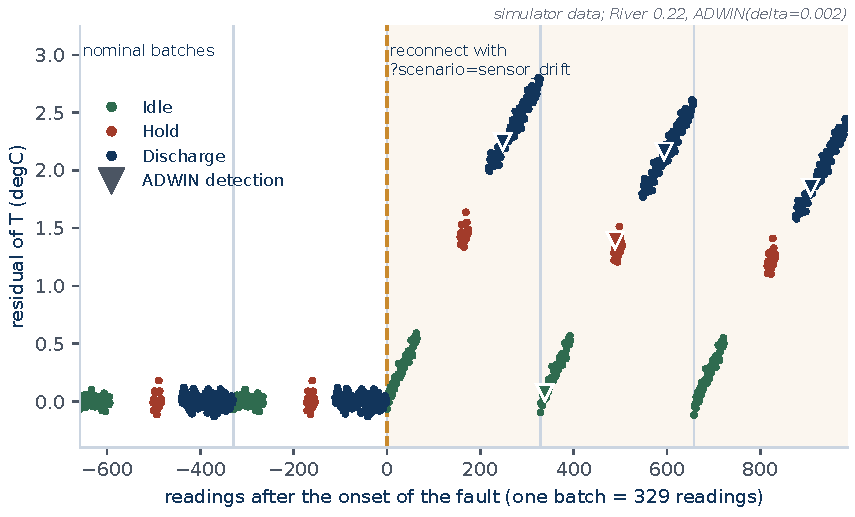
\includegraphics[width=8.2cm]{images/class30_residuals.pdf}};
\node[tileblue, anchor=north west, minimum width=5.0cm, minimum height=1.55cm, text width=4.75cm, align=left, font=\scriptsize] at (8.4,0.1) {{\bfseries\color{courseblue}\faIcon{industry}\ Class 30.} An online baseline per steady state and ADWIN on its residual detect a calibration drift of the temperature probe.};
\node[tileblue, anchor=north west, minimum width=5.0cm, minimum height=1.55cm, text width=4.75cm, align=left, font=\scriptsize] at (8.4,-1.6) {{\bfseries\color{courseblue}\faIcon{desktop}\ \texttt{App\_Stream.py}.} The same pattern on a live weather stream: online regression, MAE, and ADWIN change points.};
\node[tilegold, anchor=north west, minimum width=5.0cm, minimum height=1.0cm, text width=4.75cm, align=left, font=\scriptsize] at (8.4,-3.3) {{\bfseries\goldink The value.} The alert is tied to live behavior, not to an offline chart.};
\end{tikzpicture}
\coursefooter
\end{cframe}

% ================================================================== PART 3
\sectiondivider{3}{Response}{first-aid}{a detection may be data drift, concept drift, or a pipeline defect; several signals are needed to tell them apart.}{$\bullet$\ Diagnose, then respond\\[3pt]$\bullet$\ Performance over time, beyond accuracy\\[3pt]$\bullet$\ Champion-challenger comparison}

\begin{cframe}{After detection: diagnose, then respond}{\cterm{Recalibration}{adjusting the mapping from scores to probabilities or decisions without retraining the model.}\cterm{Rollback}{returning to an earlier, known-good version.}}
\centering
\begin{tikzpicture}
\foreach \i/\col/\ico/\ttl/\txt in {0/coursered/plug/Verify/{Rule out ingestion and schema defects.}, 1/coursegold/stethoscope/Diagnose/{Temporary, seasonal, or structural?}, 2/coursegreen/tools/Respond/{The lightest response that removes the risk.}, 3/courseblue/clipboard-list/Record/{Log the event, decision, and evidence.}} {
  \pgfmathsetmacro{\x}{\i*3.4}
  \node[tile, fill=white, draw=\col, thick, anchor=north west, minimum width=3.2cm, minimum height=2.2cm] at (\x,0) {};
  \node[circle, fill=\col, text=white, minimum size=0.55cm, inner sep=0, font=\small\bfseries] at (\x+0.42,-0.42) {\the\numexpr\i+1\relax};
  \node[text=\col!70, font=\Large] at (\x+2.75,-0.42) {\faIcon{\ico}};
  \node[anchor=north west, font=\footnotesize\bfseries, text=courseblue, inner sep=0pt] at (\x+0.2,-0.85) {\ttl};
  \node[anchor=north west, text width=2.85cm, align=left, font=\scriptsize, inner sep=0pt] at (\x+0.2,-1.2) {\txt};
}
\foreach \x in {3.2,6.6,10.0} {\draw[arrowgold] (\x,-0.42) -- (\x+0.2,-0.42);}
\node[anchor=west, font=\tiny\bfseries, text=coursegray] at (0,-2.5) {POSSIBLE RESPONSES, FROM THE LIGHTEST};
\foreach \x/\ico/\t in {0/user-check/Human review, 2.25/sliders-h/Change thresholds, 4.5/balance-scale/Recalibrate, 6.75/redo-alt/Retrain, 9.0/exchange-alt/Switch model, 11.25/undo/Roll back} {
  \node[chip, anchor=north west, minimum width=2.15cm, minimum height=0.55cm, font=\tiny\bfseries, align=center] at (\x,-2.7) {\faIcon{\ico}\ \t};
}
\keyidea{-3.65}{Retraining is one response among six, and rarely the first: a response without a diagnosis can bake a defect into the next model.}
\end{tikzpicture}
\coursefooter
\end{cframe}

\begin{cframe}{Performance over time, beyond accuracy}{\cterm{Alert fatigue}{the loss of attention caused by too many alerts, most of them irrelevant.}}
\centering
\begin{tikzpicture}
\infotile{0}{0}{6.6}{1.55}{tileblue}{courseblue}{brain}{Model metrics}{Precision, recall, AUC, MAE, as labels arrive.}
\infotile{6.8}{0}{6.6}{1.55}{tileblue}{courseblue}{tachometer-alt}{Operational metrics}{Latency, queue length, failed predictions.}
\infotile{0}{-1.7}{6.6}{1.55}{tilegold}{coursegold}{briefcase}{Business metrics}{Intervention yield, review load, alert fatigue.}
\infotile{6.8}{-1.7}{6.6}{1.55}{tilegreen}{coursegreen}{user-friends}{Human signals}{Overrides, complaints, and losses of trust.}
\keyidea{-3.55}{Plot every metric against time: a single number hides the trend, and the trend is what reveals drift.}
\end{tikzpicture}
\coursefooter
\end{cframe}

\begin{cframe}{Champion-challenger comparison}{\cterm{Shadow mode}{the challenger receives live inputs and predicts, but its predictions are not used.}}
\centering
\begin{tikzpicture}
\node[chip, minimum width=2.3cm, minimum height=1.0cm, font=\scriptsize\bfseries] (traffic) at (1.15,-1.2) {\faIcon{exchange-alt}\ Live traffic};
\node[tile, fill=white, draw=coursegreen, very thick, minimum width=3.2cm, minimum height=1.0cm, font=\scriptsize, align=center] (champ) at (5.3,-0.45) {{\bfseries\color{courseblue}\faIcon{trophy}\ Champion}\\serves every decision};
\node[tile, fill=white, draw=coursegray!70, thick, dashed, minimum width=3.2cm, minimum height=1.0cm, font=\scriptsize, align=center] (chall) at (5.3,-1.95) {{\bfseries\color{courseblue}\faIcon{user-secret}\ Challenger}\\shadow, or sampled traffic};
\node[tilegold, minimum width=3.2cm, minimum height=1.6cm, font=\scriptsize, align=center, text width=2.9cm] (cmp) at (9.6,-1.2) {{\bfseries\goldink\faIcon{chart-line}\ Comparison over time}\\on the same inputs, as labels arrive};
\node[chip, fill=coursegreen, minimum width=1.9cm, minimum height=1.0cm, font=\scriptsize\bfseries, align=center] (dec) at (12.45,-1.2) {Promote\\or keep};
\draw[arrowgold] (traffic.east) -- (champ.west);
\draw[arrowgold] (traffic.east) -- (chall.west);
\draw[arrowgray] (champ.east) -- (cmp.west);
\draw[arrowgray] (chall.east) -- (cmp.west);
\draw[arrowgray] (cmp.east) -- (dec.west);
\node[tileblue, anchor=north west, minimum width=6.6cm, minimum height=1.15cm, text width=6.2cm, align=left, font=\scriptsize] at (0,-2.85) {{\bfseries\color{courseblue}Why over time.} One lucky offline result is not evidence; a sustained advantage on live inputs is.};
\node[tileblue, anchor=north west, minimum width=6.6cm, minimum height=1.15cm, text width=6.2cm, align=left, font=\scriptsize] at (6.8,-2.85) {{\bfseries\color{courseblue}When it helps most.} Concept drift is suspected but labels are delayed (Class 27, evaluation gates).};
\end{tikzpicture}
\coursefooter
\end{cframe}

% ================================================================== PART 4
\sectiondivider{4}{Scalability}{server}{a detection leads to a diagnosis, then to the lightest response that removes the risk.}{$\bullet$\ From watching the system to sizing it\\[3pt]$\bullet$\ Horizontal scaling and its trade-offs\\[3pt]$\bullet$\ The classroom simulator as a case}

\begin{cframe}{From watching the system to sizing it}{\cterm{Throughput}{the number of requests or samples processed per unit of time.}}
\centering
\begin{tikzpicture}
\node[anchor=west, font=\tiny\bfseries, text=coursegray] at (0,0.15) {LOAD CAN GROW ALONG FOUR DIMENSIONS};
\foreach \i/\ico/\ttl/\txt in {0/bolt/Requests per second/{A transaction spike on the fraud API.}, 1/layer-group/Batch size/{More samples scored in one call.}, 2/stream/Number of streams/{More plants, more sensors per plant.}, 3/desktop/Simultaneous clients/{Many dashboards reading one stream.}} {
  \pgfmathsetmacro{\x}{\i*3.4}
  \node[tile, fill=white, draw=courseblue!60, thick, anchor=north west, minimum width=3.2cm, minimum height=1.75cm] at (\x,-0.05) {};
  \node[text=courseblue!70, font=\Large] at (\x+1.6,-0.45) {\faIcon{\ico}};
  \node[font=\scriptsize\bfseries, text=courseblue] at (\x+1.6,-0.9) {\ttl};
  \node[anchor=north, text width=2.9cm, align=center, font=\scriptsize, inner sep=0pt] at (\x+1.6,-1.1) {\txt};
}
\node[tile, fill=courseice, anchor=north west, minimum width=13.4cm, minimum height=0.8cm, text width=13.0cm, align=left, font=\scriptsize] at (0,-2.05) {{\bfseries\color{courseblue}\faIcon{heartbeat}\ Monitoring and scaling meet.} Monitoring shows that the system behaves correctly; scalability asks whether it keeps doing so under more load.};
\warning{-3.1}{exclamation-triangle}{A failed system.}{A model that is accurate but too slow or too expensive under load is still a failed system.}
\end{tikzpicture}
\coursefooter
\end{cframe}

\begin{cframe}{Horizontal scaling for a serving layer}{\cterm{Stateless replica}{a copy of the service that keeps no client state, so any copy can answer any request.}\cterm{Autoscaling}{adding or removing replicas automatically from a load signal.}}
\centering
\begin{tikzpicture}
\node[chip, minimum width=1.8cm, minimum height=0.9cm, font=\scriptsize\bfseries] (client) at (0.9,-1.55) {\faIcon{users}\ Clients};
\node[tilegold, minimum width=2.1cm, minimum height=1.1cm, font=\scriptsize, align=center] (lb) at (3.8,-1.55) {{\bfseries\goldink\faIcon{random}}\\Load balancer};
\foreach \k/\y in {1/-0.3, 2/-1.55, 3/-2.8} {
  \node[tile, fill=white, draw=courseblue, thick, minimum width=2.3cm, minimum height=0.8cm, font=\scriptsize] (r\k) at (7.0,\y) {\faIcon{server}\ Replica \k};
  \draw[arrowgold] (lb.east) -- (r\k.west);
}
\node[tileblue, minimum width=2.7cm, minimum height=1.3cm, font=\scriptsize, align=center, text width=2.5cm] (store) at (11.4,-1.55) {{\bfseries\color{courseblue}\faIcon{archive}\ Model registry}\\one versioned artifact};
\foreach \k in {1,2,3} {\draw[arrowgray] (r\k.east) -- (store.west);}
\draw[arrowgold] (client) -- (lb);
\keyidea{-3.6}{Stateless replicas behind a load balancer are the standard pattern; each loads the same versioned artifact, and autoscaling follows queue depth or CPU load.}
\end{tikzpicture}
\coursefooter
\end{cframe}

\begin{cframe}{Cost-latency trade-offs}{\cterm{Cold start}{the delay of the first request served by a replica that has just been started.}}
\centering
\begin{tikzpicture}
\node[chip, fill=coursegreen, anchor=north west, minimum width=4.9cm, minimum height=0.42cm, font=\tiny\bfseries] at (3.55,0) {WHAT IT GAINS};
\node[chip, fill=coursered, anchor=north west, minimum width=4.8cm, minimum height=0.42cm, font=\tiny\bfseries] at (8.6,0) {WHAT IT COSTS};
\traderow{-0.55}{clone}{More replicas}{Lower latency under load.}{Higher infrastructure cost.}
\traderow{-1.25}{compress-alt}{Smaller batch size}{Lower latency per request.}{Lower throughput per instance.}
\traderow{-1.95}{expand-arrows-alt}{Larger instance}{Room for larger models.}{Higher cost while idle.}
\traderow{-2.65}{memory}{Prediction caching}{No recomputation for repeated inputs.}{Risk of stale predictions.}
\traderow{-3.35}{inbox}{Queued inference}{Smooths load spikes.}{Adds response delay.}
\keyidea{-4.15}{Every lever moves cost, latency, or freshness; state the service-level objective first, then choose the lever.}
\end{tikzpicture}
\coursefooter
\end{cframe}

\begin{cframe}{Case: the classroom simulator}{\cterm{Global clock}{a design in which each served value is a function of the wall-clock time, not of the client.}}
\centering
\begin{tikzpicture}
\infotile{0}{0}{6.6}{2.25}{tilegreen}{coursegreen}{clock}{Designed to scale out}{Each reading is a function of the wall clock (\texttt{\_global\_event\_id} in \texttt{serving.py}). With no client state, any replica serves every team the same reading.}
\infotile{6.8}{0}{6.6}{2.25}{tileblue}{courseblue}{heartbeat}{Observable}{\texttt{/health} reports status and speed; \texttt{/schema} states the contract. A dashboard can show staleness when events stop.}
\infotile{0}{-2.4}{6.6}{1.65}{tilegold}{coursegold}{snowflake}{A real latency to explain}{A free hosting plan may suspend an idle service: the next client waits for a cold start.}
\infotile{6.8}{-2.4}{6.6}{1.65}{tilered}{coursered}{exclamation-triangle}{An honest gap}{No load-testing exercise exists yet: a candidate for a project or submodule.}
\keyidea{-4.25}{Scalability is a property to design for: the global clock made scaling out possible before any load arrived.}
\end{tikzpicture}
\coursefooter
\end{cframe}

\begin{cframe}{Discussion prompt}{\cterm{Load test}{a controlled experiment that measures the behavior of a service under a defined load.}}
\centering
\begin{tikzpicture}
\node[tilegold, anchor=north west, minimum width=13.4cm, minimum height=1.9cm] at (0,0) {};
\badge{0.75}{-0.95}{coursegold}{comments}
\node[anchor=west, text width=11.4cm, align=left] at (1.5,-0.95) {{\bfseries\tiny\goldink QUESTION}\\[3pt]{\bfseries\large\color{courseblue}The fraud API is correct and well monitored at 10 requests per second. What breaks first at 10{,}000, and how would you know before production does?}};
\infotile{0}{-2.15}{6.6}{1.75}{tileblue}{courseblue}{link}{Why this question}{It connects monitoring evidence to scaling decisions.}
\infotile{6.8}{-2.15}{6.6}{1.75}{tileblue}{courseblue}{vial}{What it motivates}{Load testing as a form of validation, with its own acceptance criteria.}
\end{tikzpicture}
\coursefooter
\end{cframe}

% ------------------------------------------------------------------ closing
\section{Wrap-up}\gdef\currentsectionname{Wrap-up}
\begin{frame}{From this class to the next}
\centering
\begin{tikzpicture}
\foreach \i/\lab/\bg/\fg in {1/Problem/courseice/coursegray, 2/Data/courseice/coursegray, 3/Features/courseice/coursegray, 4/Model/courseice/coursegray, 5/Interface/courseice/coursegray, 6/Delivery/courseblue!22/courseblue, 7/Monitor/courseblue/white, 8/Evolution/courseblue/white} {
  \node[rounded corners=3pt, minimum width=1.55cm, minimum height=0.6cm, font=\scriptsize\bfseries, fill=\bg, text=\fg] at ({0.78+(\i-1)*1.68},0) {\lab};
}
\node[font=\tiny\bfseries, text=courseblue] at (6.7,-0.52) {THIS CLASS CLOSES THE LIFECYCLE: OPERATION AND EVOLUTION UNDER REAL LOAD};
\foreach \x/\sty/\ico/\ttl/\txt in {0/tileblue/lightbulb/What stays with us/{$\bullet$\ Monitor four layers, not one.\\[3pt]$\bullet$\ Diagnose before responding.\\[3pt]$\bullet$\ Design for scale before the load arrives.}, 4.55/tileblue/project-diagram/Use it in your project/{$\bullet$\ Name one signal per layer, and its threshold.\\[3pt]$\bullet$\ Say which component breaks first under ten times the load.}, 9.1/tilegold/arrow-right/Next: Class 34/{\textbf{Practical project: brainstorm.}\\[3pt]Teams scope their own project with the full lifecycle in view, from requirements to monitoring.}} {
  \node[\sty, anchor=north west, minimum width=4.3cm, minimum height=3.8cm] at (\x,-0.95) {};
  \badge{\x+0.65}{-1.6}{courseblue}{\ico}
  \node[anchor=west, text width=3.0cm, align=left, font=\small\bfseries, text=courseblue] at (\x+1.2,-1.6) {\ttl};
  \node[anchor=north west, text width=3.9cm, align=left, font=\scriptsize] at (\x+0.2,-2.25) {\txt};
}
\node[tilegold, fill=white, anchor=north west, minimum width=13.4cm, minimum height=0.95cm, text width=12.6cm, align=left, font=\footnotesize] at (0,-5.0) {{\bfseries\goldink\faIcon{route}\ Course thread.} Every architecture, model, interface, and process choice should support sustainable evolution under real, growing use.};
\end{tikzpicture}
\coursefooter
\end{frame}

% ------------------------------------------------------------------ references
\begin{frame}{Papers and materials}
\centering
\begin{tikzpicture}
\refrow{0}{2.55}{search}{Drift detection}{Gama, J., \v{Z}liobait\.{e}, I., Bifet, A., Pechenizkiy, M., and Bouchachia, A. (2014). A survey on concept drift adaptation. \emph{ACM Computing Surveys}, 46(4), 44:1--44:37.\\Bifet, A. and Gavald\`a, R. (2007). Learning from time-changing data with adaptive windowing. \emph{SIAM SDM}, 443--448.\\Page, E. S. (1954). Continuous inspection schemes. \emph{Biometrika}, 41(1/2), 100--115.}
\refrow{-2.55}{1.75}{file-alt}{ML in production}{Sculley, D. et al. (2015). Hidden technical debt in machine learning systems. \emph{NeurIPS}.\\Breck, E., Cai, S., Nielsen, E., Salib, M., and Sculley, D. (2017). The ML test score: a rubric for ML production readiness and technical debt reduction. \emph{IEEE International Conference on Big Data}.}
\refrow{-4.3}{1.0}{book}{Books}{Huyen, C. (2022). \emph{Designing Machine Learning Systems}. O'Reilly.\\Beyer, B., Jones, C., Petoff, J., and Murphy, N. R. (2016). \emph{Site Reliability Engineering}. O'Reilly.}
\refrow{-5.3}{0.6}{link}{Guides}{\href{https://12factor.net/}{The Twelve-Factor App}; \href{https://prometheus.io/docs/introduction/overview/}{Prometheus overview}; \href{https://docs.evidentlyai.com/}{Evidently}; \href{https://riverml.xyz/latest/api/drift/ADWIN/}{River ADWIN}.}
\end{tikzpicture}
\coursefooter
\end{frame}

\end{document}
